\newpage
\exer{10}


\textbf{\underline{ex10.html}}
\vspace{0.1cm}

\lstinputlisting[style=htmlstyle]{Code/EX10/ex10.html}

\vspace{1.25cm}

\textbf{\underline{Output}}

\vspace{0.1cm}
\begin{center}
\setlength{\fboxrule}{2pt} % Set border thickness
\fbox{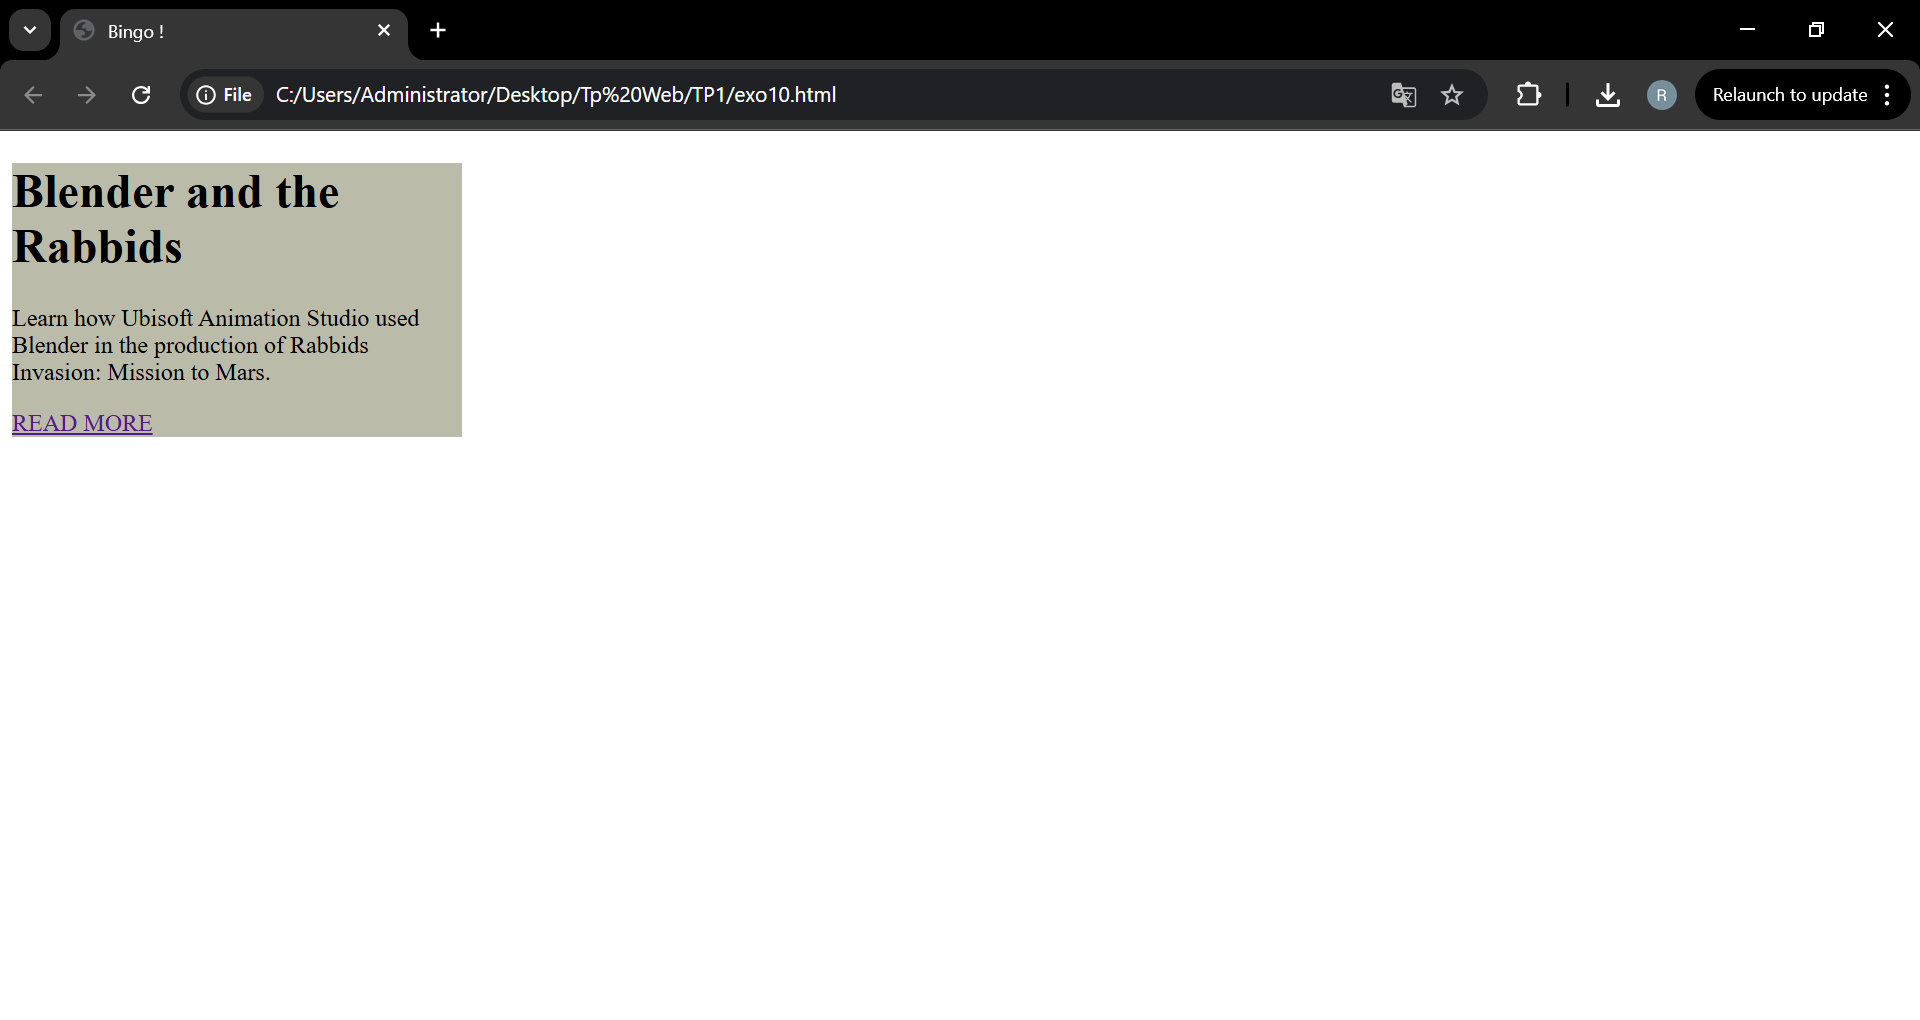
\includegraphics[height=0.4\textheight]{Code/EX10/ex10.PNG}}
\end{center}

\vspace{0.25cm}
\begin{prettyBox}{Utilite}{myblue}
L'utilite des \(<\)div\(>\) est de regroupe des elements , et 
leur applique le meme style
\end{prettyBox}
